% #############################################################################
% This is Chapter 4
% !TEX root = ../main.tex
% #############################################################################
% Change the Name of the Chapter i the following line
\fancychapter{Evaluation}
\cleardoublepage
% The following line allows to ref this chapter
\label{chap:evaluation}
This chapter describes the methodology adopted to test the Power Share mobile application with real users. Data resulting from the users’ test are presented. 

\section{Methodology}

The evaluation of Power Share app has three main goals:


\begin{enumerate}
    \item Assessing the usability of the system;
    \item Assessing users acceptance of \ac{ET} in Madeira Island to understand if it could be a viable future business model for the SMILE project;
    \item Evaluating users understanding and attitudes toward adoption of blockchain as a payment method.
\end{enumerate}


The methodology selected for assessing the aspects mentioned above includes semi-structured interviews (to be performed after the one-month test) and monitoring users’ interactions through the Fabric.io platform. Due to time constraints, the start of the field test has been postponed thus, results from the semi-structured interviews cannot be included in the present document (but will be presented during the viva). 


\subsection{Semi-structured interviews}

The interviews with the participants in the field test are scheduled to start mid-October. Each interview should last around one hour and will be performed with the support of researchers from the Madeira-Interactive Technologies Institute.
The main topics to be covered during the interviews are:
\begin{itemize}
    \item Understanding and perception of the system (e.g. perceived usefulness);
    \item Actual use (i.e. how they used the app);
    \item Behavioral intention (i.e. their willingness to use the app/system in the future);
    \item Usability (e.g. perceived ease to use);
    \item Their perception of using blockchain as a payment method.
\end{itemize}

\subsection{Monitoring users’ interactions}

To further understand how participants used the application, their interactions have been monitored using Fabric.io. 


Specifically, data collected concern:
\begin{enumerate}
    \item \textbf{Daily usage of the application:} number of daily interactions, which features they accessed and at what time;
    \item \textbf{Performance of the app:} i.e. crashes;
    \item \textbf{Trading settings:} if and how users set criteria for buying and selling energy;
\end{enumerate}

\subsection{Procedure}

To assess the system, we decided to run a small pilot in Madeira island, asking prosumers to use the application for a month. Initially, ten households in Funchal were recruited, but at the end, only nine of them participated in the field test (one decided to withdraw his participation).
 Before performing the study, informed consent was provided to participants. Then the research team, supported by local technicians, verified the existing communication infrastructure (internet connection) and installed the required equipment to collect production and consumption data (smart meters). Also, an Android tablet was provided to those participants that did not have a mobile device able to run the app.

At the end of August, an email with instructions to download and install the app was sent to all participants. The application was launched on September 1st. Not all users installed the app immediately, thus a reminder email was sent to those users who still had to create an account.
 Every weekend, each user received via email a summary of his weekly production and consumption breakdown (an example of the weekly summary can be founded in the \cref{chapter:appendixC}).
 
 \section{Results}
 As expected, data collected through Fabric.io (\cref{fig:gr1}) show that the most used feature was the home (real-time feedback). According to the literature on \ac{EF}, real-time feedback is the information users are more interested in, thus the application was designed to show this screen by default every time a user launches the app. For this reason, the high score of real-time feedback (which was used over 100\% times more than the second most used feature) is not enough to confirm users interest for it and thus needs to be addressed during the interviews. Interestingly, the second most popular feature was the ranking. This result supports findings from previous studies on \ac{EF}, which demonstrate the effectiveness of social comparison. “Ranking” is followed by  “Histórico” (self-comparison). On this respect, it should be pointed out that daily and weekly data received more or less the same attention from users, while monthly data was not very popular (likely because the study lasted only one month).


Despite most of the users selected the “automatic settings” for trading energy,  they did access trading settings and a list of transactions several times. This result suggests a certain degree of curiosity from users about \ac{ET}, which definitely has to be further investigated during the interviews. Another interesting result is the lack of interest in the “IOTA wallet”, which was the less popular feature together with “account settings”. This could be due to the fact that both “IOTA wallet” and “account settings” were hidden compared to the other features of the app since accessible only from the overflow menu placed in the top app bar. Nevertheless, this result needs to be further investigated during the interviews since it could represent a lack of interest or understanding of payment via blockchain. 

 
 \begin{figure}[h]
\centering
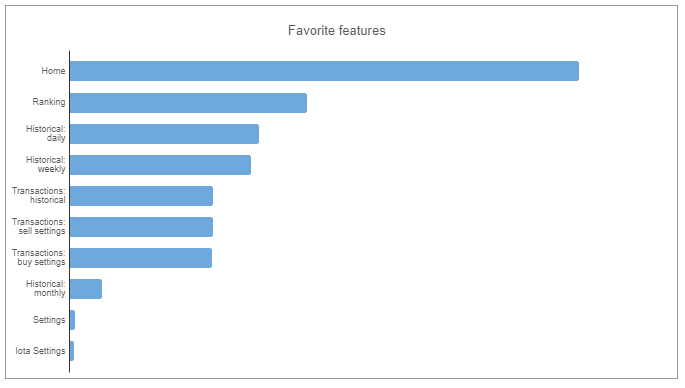
\includegraphics[width=0.8\textwidth]{./Images/graph1}
\caption{Favorite features based in the number of accesses}
\label{fig:gr1}
\end{figure}

Users motivations behind results reported above will be investigated during the interviews. Especially, what needs to be clarified is the reason that led the majority of users to select the “automatic settings” for trading energy, since it could be due to a usability issue (during the pilot test, the manual setting task was defined as the most demanding).  

\Cref{fig:gr2} shows the number of accesses to the app throughout the study. No significant correlation has been found between the number of accesses and day of the week (included weekend vs. weekdays). Also, surprisingly, push notifications and weekly summary did not affect the use of the app.. 


 \begin{figure}[h]
\centering
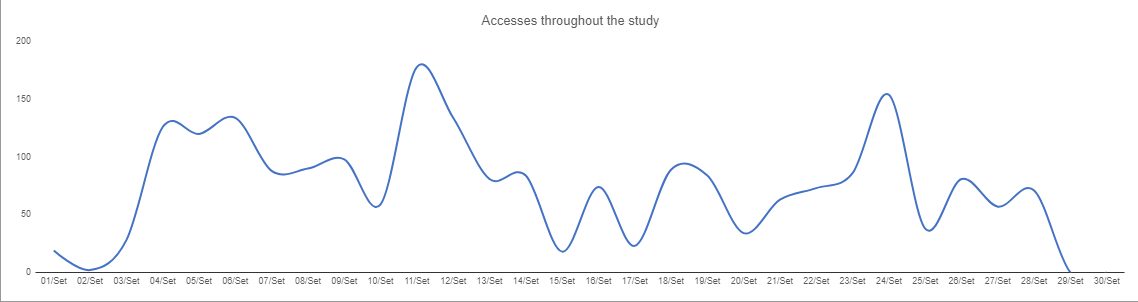
\includegraphics[width=0.8\textwidth]{./Images/graph2}
\caption{Application accesses throughout the study }
\label{fig:gr2}
\end{figure}

Each user’s session lasted an average of 2 minutes and 15 seconds. In agreement with the literature on EF, interaction with the system decreased over time (\cref{fig:gr3}). 


 \begin{figure}[h]
\centering
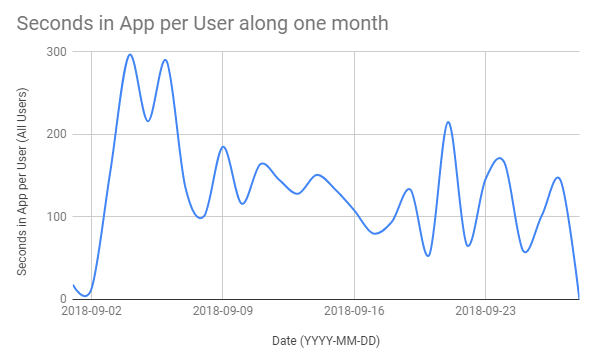
\includegraphics[width=0.8\textwidth]{./Images/graph3}
\caption{Seconds in the Application throughout the study}
\label{fig:gr3}
\end{figure}

Regarding the \ac{ET} (\cref{tab:tr}), we recorded a daily average of 19 transactions, which means more than 2 transactions a day per user. 
At the end of the study, a total of 349 transactions were performed, the corresponding to about 45.1 kWh of energy shared between the users. 



The main bottlenecks identified regard the payment system. As already explained in 3.2.2, to pay for the energy received, users have to press the “pagar as minhas despesas” button in their “IOTA wallet”. In the server, a transaction could have three different states: “not-attached” (not paid), “attached” (after the user presses the pay button), and “validated” (when the payment is performed successfully). At the end of the study, all transactions were “not-attached”, which means that none of the users have understood they were required to allow the payment manually. The choice of recording the “attached” state is due to the fact that the payment through IOTA is very slow, which could, therefore, lead the user to close the application before the process is completed (thus leading to interrupt the payment). By recording this intermediate state, we have been able to verify if users tried to make payments. In addition, none of the users have generated the destination addresses, which are required to receive a payment. These two bottlenecks suggest the need to redesign the payment process by increasing the level of automation and/or adding affordances to help users performing the required actions.

\begin{table}[htb]
\centering
\normalsize
    \caption{Transactions data during the study}
    \label{tab:tr}
{\footnotesize
    \begin{tabular}{ | c | c | c | c | }
    \hline 
    	& \textbf{Nr Transactions} & \textbf{Ammount (\euro)} & \textbf{Ammount (kWh)}\\ \hline \hline
    Average  & 19.4  &  0.41  &   2.51 \\ \hline
    Max  & 34   &  0.81  &   4.96 \\ \hline 
    Min  & 9   &  0.15  &   0.93 \\ \hline
    Total  & 349  &  7.35  & 45.12 \\ \hline
    \end{tabular}
    }
\end{table}

Throughout the study, only one crash occurred, which affected three users (\cref{fig:crash}). This crash was due to the fact that those users have run a query at midnight; in other words, they were asking the server for data with wrong intervals, thus the server returned an error and the application crashed.

 \begin{figure}[h]
\centering
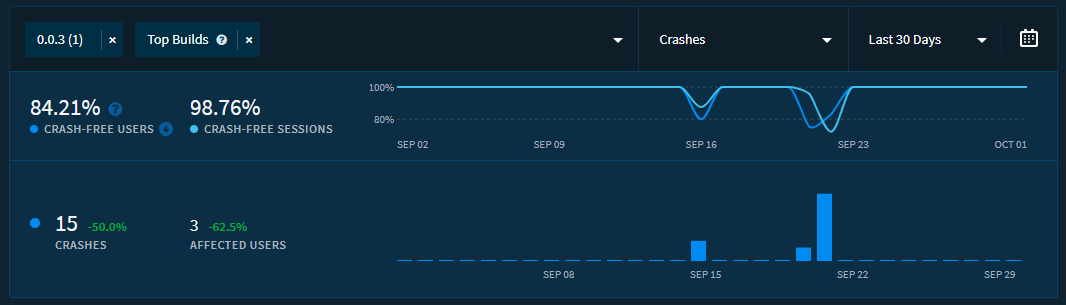
\includegraphics[width=0.8\textwidth]{./Images/crash}
\caption{Application crashes during the deployment}
\label{fig:crash}
\end{figure}